\section{Design}
\label{sec:Design}

\subsection{Architecture Design}
Because we selected the web application model from the beginning, so the classic client-server architecture was quickly adopted, which is a distributed application structure that partitions tasks or workloads between the providers of a resource or service, called servers, and service requesters, called clients. In theory, any device connected to the Internet can try to access and obtain the resources or services of the server while the server is running normally. Figure \ref{Client-Server Architecture} shows how it works.

\begin{figure}[htb]
\centering
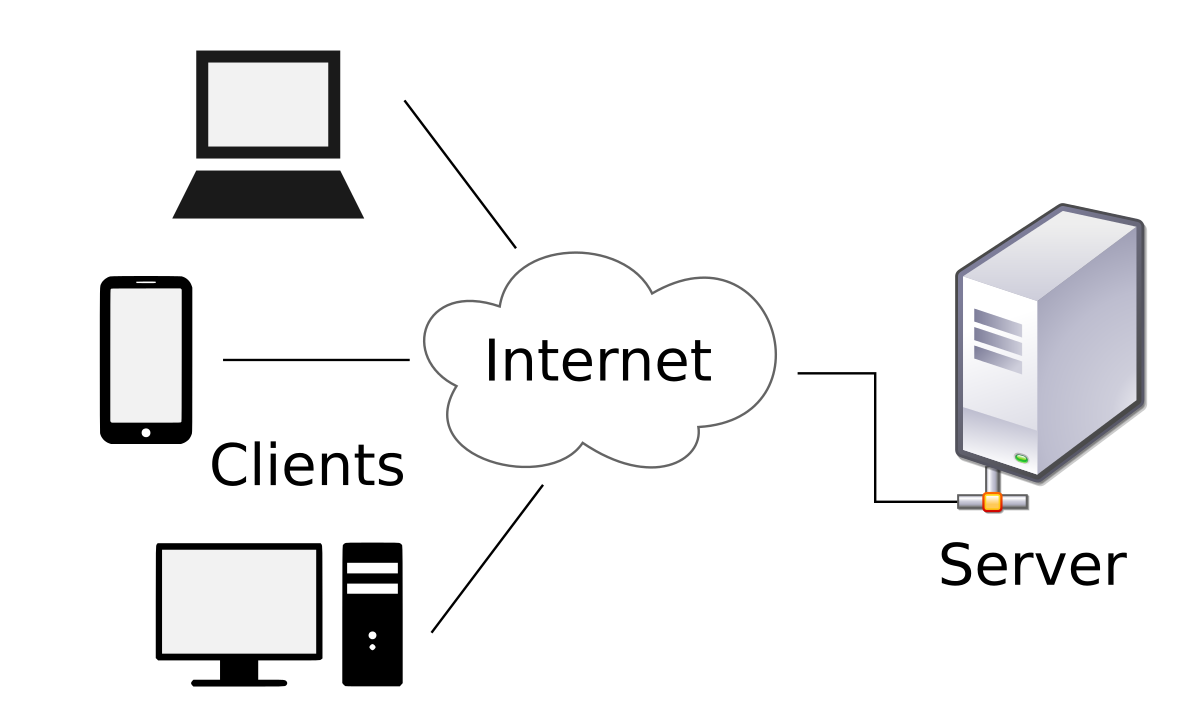
\includegraphics[width=\textwidth]{section03/assets/client_server.png}
\caption[the Architecture of Client-Server Model]{\label{Client-Server Architecture}the Architecture of Client-Server Model}
\end{figure}

Based on the client-server structure, we have detailed its component structures below:
\subsubsection{Web Browser or Client}
The web browser or client is the interface rendition of a web app functionality, with which the user interacts with. This content delivered to the client can be developed using HTML, JavaScript, and CSS and doesn’t require operating system related adaptations. In essence, the web browser or client manages how end users interact with the application.

There are three, well-known Web Application Architecture types available in the modern tech landscape: Single Page Applications (SPA), Microservices, and Serverless Architectures. Considered the needs of the project and the choice of the Software Development Life Cycle (SDLC) model, we chose the SPA architecture.

The SPA model interacts with the user in a more dynamic fashion by providing updated content within the current page, rather than loading entirely new pages from the server with each action from the user. It helps prevent interruptions in the user experience, transforming the behavior of the application such that it resembles a traditional desktop application.

\subsubsection{Web Application Server}
The web application server manages business logic and data persistence and can be built using PHP, Python, Java, Ruby, .NET, Node.js, among other languages. It’s comprised of at least a centralized hub or control center to support multi-layer applications. The essential purpose of a web server architecture is to complete requests made by clients for a website. The clients are typically browsers and mobile apps that make requests using secure HTTPs protocol, either for page resources or a REST API.

Since the focus of this project is on the client side (frontend), which is the map generator (written in JavaScript), so we chose the Node.js Express framework. Moreover, the Node.js is written using JavaScript and is the same technology as frontend components, which makes it easier for the developer to program backend services and frontend user interfaces. It also provides consistency, code sharing and reusability, simple knowledge-transfer, and a large number of free tools. These benefits bring flexibility and efficiency when building this project.

\subsubsection{Database Server}
The database server provides and stores relevant data for the application. Additionally, it may also supply the business logic and other information that is managed by the web application server. There are multiple popular database systems available: Oracle, MySQL, Microsoft SQL Server, PostgreSQL, MongoDB, MariaDB, DB2, and SAP HANA.

Because of the project involves a small number of entities and the relationships among entities are not complicated, and the choice of the Software Development Life Cycle (SDLC) model, we chose the MongoDB, which is dynamic, flexible and easy to get started. It also provides high performance, high availability, and high scalability. What's more, our main purpose is to save maps and implement basic CRUD (create, retrieve, update, delete) operations of the database. As MongoDB is a schema-less database (written in C++), we can serialize the map data to JSON, send it to MongoDB and then save it.

\subsection{Database Design}
NoSQL, which stands for "not only SQL," is an approach to database design that can accommodate a wide variety of data models, including key-value, document, columnar and graph formats. MongoDB is a type of NoSQL database. A record in MongoDB is a document, which is a data structure composed of field and value pairs. MongoDB documents are similar to JSON objects, the values of fields may include other documents, arrays, and arrays of documents.

Firstly, we thought there should be two entities: the user and the map. A user can have many maps, but a map can only belong to one user. Thus, the relationship between the user and the map should be One-to-Many.

MongoDB provides two ways of data modeling: Embedded Data Modeling and Normalized Data Modeling. Using Embedded Data Modeling, we may embed related data in a single structure or document, which means we should store maps in the user schema. But the data of the map is relatively large, in general, the CRUD operations will be slower, and the map cannot exist as a separate entity, so this one is beyond our consideration.

Normalized Data Modeling provides One-to-One relationship and One-to-Many relationship,
here we chose the Normalized One-to-Many structure.

Figure \ref{ER Diagram} shows the relationship between the ``user'' and the ``map''.

\begin{figure}[htb]
\centering
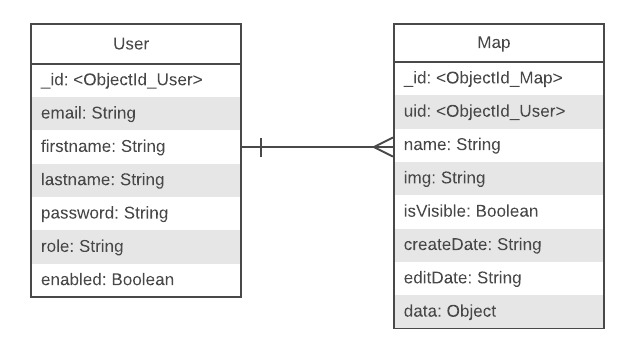
\includegraphics[width=\textwidth]{section03/assets/ER_Diagram.png}
\caption[ER Diagram]{\label{ER Diagram}ER Diagram}
\end{figure}

\subsection{REST API Design}
REST is the acronym for Representational State Transfer. It is an architectural style for distributed hypermedia systems and was first presented by Roy Fielding in 2000 in his famous dissertation.
%[https://www.ics.uci.edu/~fielding/pubs/dissertation/rest_arch_style.htm]

Like any other architectural style, REST also does have it’s own 6 guiding constraints which must be satisfied if an interface needs to be referred as RESTful. These principles are listed below:
\begin{enumerate}
  \item Client–server - By separating the user interface concerns from the data storage concerns, we improve the portability of the user interface across multiple platforms and improve scalability by simplifying the server components
  \item Stateless - Each request from a client to server must contain all of the information necessary to understand the request, and cannot take advantage of any stored context on the server. Session state is therefore kept entirely on the client
  \item Cacheable – Cache constraints require that the data within a response to a request be implicitly or explicitly labeled as cacheable or non-cacheable. If a response is cacheable, then a client cache is given the right to reuse that response data for later, equivalent requests
  \item Uniform interface – By applying the software engineering principle of generality to the component interface, the overall system architecture is simplified and the visibility of interactions is improved.
  \item Layered system – The layered system style allows an architecture to be composed of hierarchical layers by constraining component behavior such that each component cannot ``see'' beyond the immediate layer with which they are interacting
  \item Code on demand (optional) – REST allows client functionality to be extended by downloading and executing code in the form of applets or scripts. This simplifies clients by reducing the number of features required to be pre-implemented
\end{enumerate}

Based on these principles, we have designed the APIs shown in Table \ref{REST API Design Table}.
\begin{table}[htb]
  \centering
  \begin{tabularx}{\textwidth}{>{\raggedright}cXX} % way of defining a fix columns width
    \toprule[1.5pt]
    \textbf{HTTP Verb} & \textbf{URI} & \textbf{Description}
    \\ \midrule[1.5pt]
    % POST & /metro/auth/signup & Sign up for a new account
    % \\ \midrule
    % POST & /metro/auth/login & Log in to the system
    % \\ \midrule
    % POST & /metro/auth/logout & Log out of the system
    % \\ \midrule
    GET & /metro/api/v1/users & Get a list of all users
    \\ \midrule
    GET & /metro/api/v1/users/\{id\} & Get the user with \{id\}
    \\ \midrule
    GET & /metro/api/v1/users/\{uid\}/ maps & Get a list of all maps of the user with \{uid\}
    \\ \midrule
    PATCH & /metro/api/v1/users/\{id\}/ password & Verify the password of the user with \{id\}
    \\ \midrule
    PUT & /metro/api/v1/users/\{id\}/ password & Update the password of the user with \{id\}
    \\ \midrule
    PUT & /metro/api/v1/users/\{id\}/ email & Update the email of the user with \{id\} \\ \midrule
    PUT & /metro/api/v1/users/\{id\}/ name & Update the name of the user with \{id\} \\ \midrule
    PUT & /metro/api/v1/users/\{id\}/ enabled & Update the enabled of the user with \{id\}
    \\ \midrule
    GET & /metro/api/v1/maps/\{id\} & Get the map with \{id\}
    \\ \midrule
    GET & /metro/api/v1/maps/ ?page=\{page\}\&limit=\{limit\} & Get a list of \{limit\} maps on page \{page\}
    \\ \midrule
    POST & /metro/api/v1/maps & Add a new map to the database
    \\ \midrule
    PUT & /metro/api/v1/maps/\{id\} & Update the map with \{id\}
    \\ \midrule
    DELETE & /metro/api/v1/maps/\{id\} & Delete the map with \{id\}
    \\ \bottomrule[1.5pt]
  \end{tabularx}
  \caption[REST API Design Table]{REST API Design Table}
  \label{REST API Design Table}
\end{table}

\subsection{Map Generator Design}
